\section{Results}
\label{sec:htoinv_results}

The fits of signal and background to the observed data are performed as outlined in Fig.~\ref{fig:htoinv_fit_overview}. Tabulated event counts in the signal region after the \gls{CR}-only fit are shown in Sec.~\ref{subsec:yield_tables_SR_CR_only_fit} to compare the background prediction from those regions to the observed data in the signal region. To check whether the \acrshort{sm} background by itself can accurately model the data, event yields in the signal region from the fit in the background-only hypothesis are exhibited in Sec.~\ref{subsec:yield_tables_SR_B_only_fit}. No significant excesses in the data are identified that can be plugged by signal, demonstrating that indeed the background-only fit can bring the data and \acrshort{sm} background into agreement within uncertainties. Limits can therefore be set.

In Secs.~\ref{subsec:htoinv_results_ttH} and \ref{subsec:htoinv_results_VH}, the results of the fits for the \ttH and \VH channels individually are shown in several forms: pre-fit vs. post-fit distributions in each category and \ptmiss bin; the observed upper limit on the signal strength parameter $\BRHinvFull$ at 95\,\% confidence level from the signal plus background hypothesis, accompanied by the median expected limit with 68\,\% and 95\,\% confidence level intervals from the background-only hypothesis; and profile likelihood scans as a function of the signal strength parameter. The outcome from combining both channels, yielding the final result, is given in Sec.~\ref{subsec:htoinv_combined_results}.


%=========================================================


\import{./}{yields_SR_CR_only_fit.tex}

From the fit invoking only the \glspl{CR} to scale the \acrlong{sm} background events in the signal region, a sufficient description of the data can be shown. The total \acrshort{sm} event counts in Tabs.~\ref{tab:yields_SR_CR_only_2016}, \ref{tab:yields_SR_CR_only_2017}, and \ref{tab:yields_SR_CR_only_2018}, which correspond to the 2016, 2017, and 2018 datasets, respectively, are very similar to data within uncertainties. The largest discrepancies occur, as expected, from the bins with small event counts such as in the \ttH boosted categories. However, with additional constraints provided by data and simulation in the background-only or signal plus background fits, dissimilarities can be mitigated to some extent.

\clearpage


%=========================================================


\import{./}{yields_SR_B_only_fit.tex}

\clearpage

The results of the background-only fit to data model it well, in large part. As noted above, no significant excess is observed in the data. With the \acrshort{sm} background describing the data sufficiently, only upper limits can be set on $\BRof{\higgstoinv}$. Post-fit distributions in the signal region---visualising the event counts in the Tabs.~\ref{tab:yields_SR_B_only_2016}, \ref{tab:yields_SR_B_only_2017}, and \ref{tab:yields_SR_B_only_2018}---are depicted in Secs.~\ref{sec:B_only_fit_plots_ttH_SR} and \ref{sec:B_only_fit_plots_VH_SR} for the \ttH and \VH categories, respectively. The ``pre-fit'' yields are from the results of the \gls{CR}-only fit documented in Sec.~\ref{subsec:yield_tables_SR_CR_only_fit}.

As expected, knowledge of the background and data in the signal region permits the background-only fit to model the data better than the \gls{CR}-only fit. Noticeable improvements are in the \ttH and \VH resolved categories. While small in some cases, the addition of the \acrshort{qcd} multijet background with 50\,\% uncertainty creates an additional avenue for constraining the backgrounds. Strong sensitivity translates to a small value of the expected upper limit on $\BRof{\higgstoinv}$.


%=========================================================


\subsection{Results from the \texorpdfstring{\ttH}{ttH} channel}
\label{subsec:htoinv_results_ttH}

Distributions of the yields in the signal region for 2016, 2017, and 2018 from the signal plus background fit are displayed in Fig.~\ref{fig:htoinv_mountain_range_ttH_SR_Postfit}. The \acrshort{sm} prediction from the \gls{CR}-only fit is also overlaid, denoted as ``pre-fit.'' Event counts from said fit are tabulated in the previous section. Corresponding figures for the \gls{CR} distributions from the \gls{CR}-only fit are given in Sec.~\ref{sec:pre_post_fit_plots_ttH_CRs}.

\begin{figure}[htbp]
    \centering
    \begin{subfigure}[b]{0.9\textwidth}
        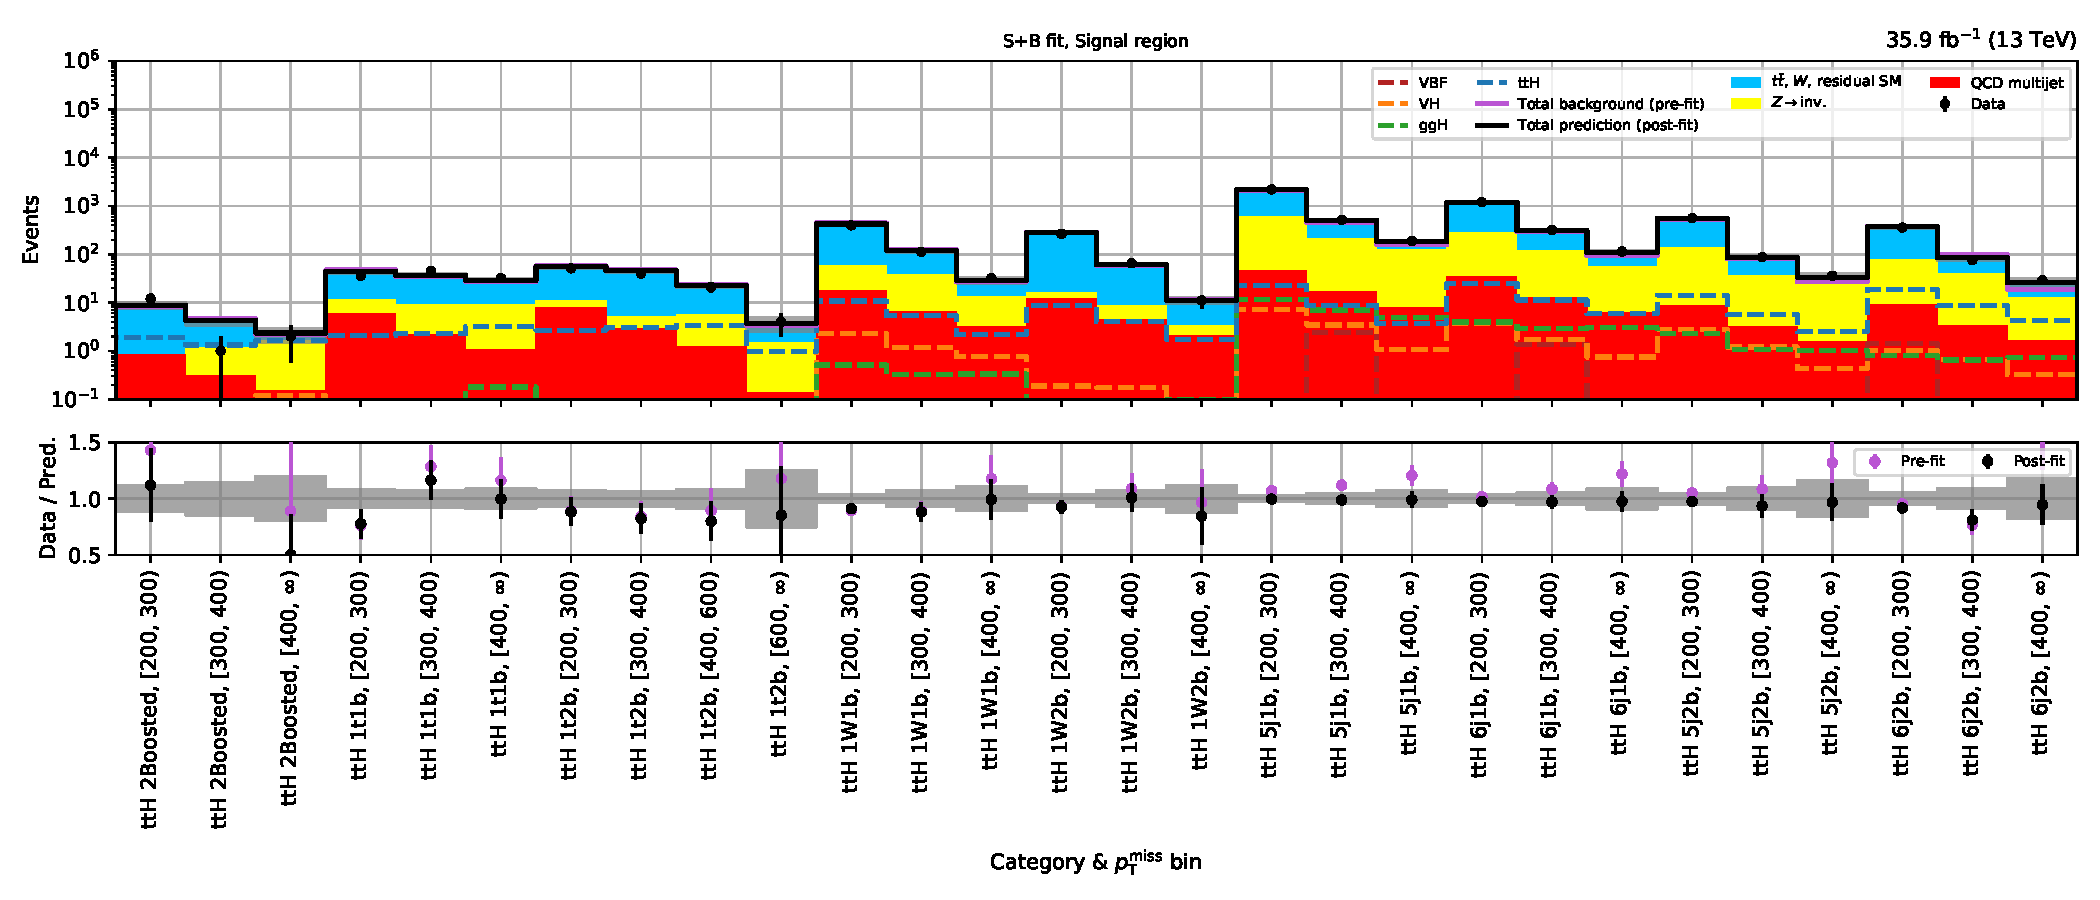
\includegraphics[width=\textwidth]{figures/mountain_ranges/2016/ttH/SR_tree_fit_s-abs_values_ttH_cats.pdf}
        \caption{\ttH --- 2016}
    \end{subfigure}

    \begin{subfigure}[b]{0.9\textwidth}
        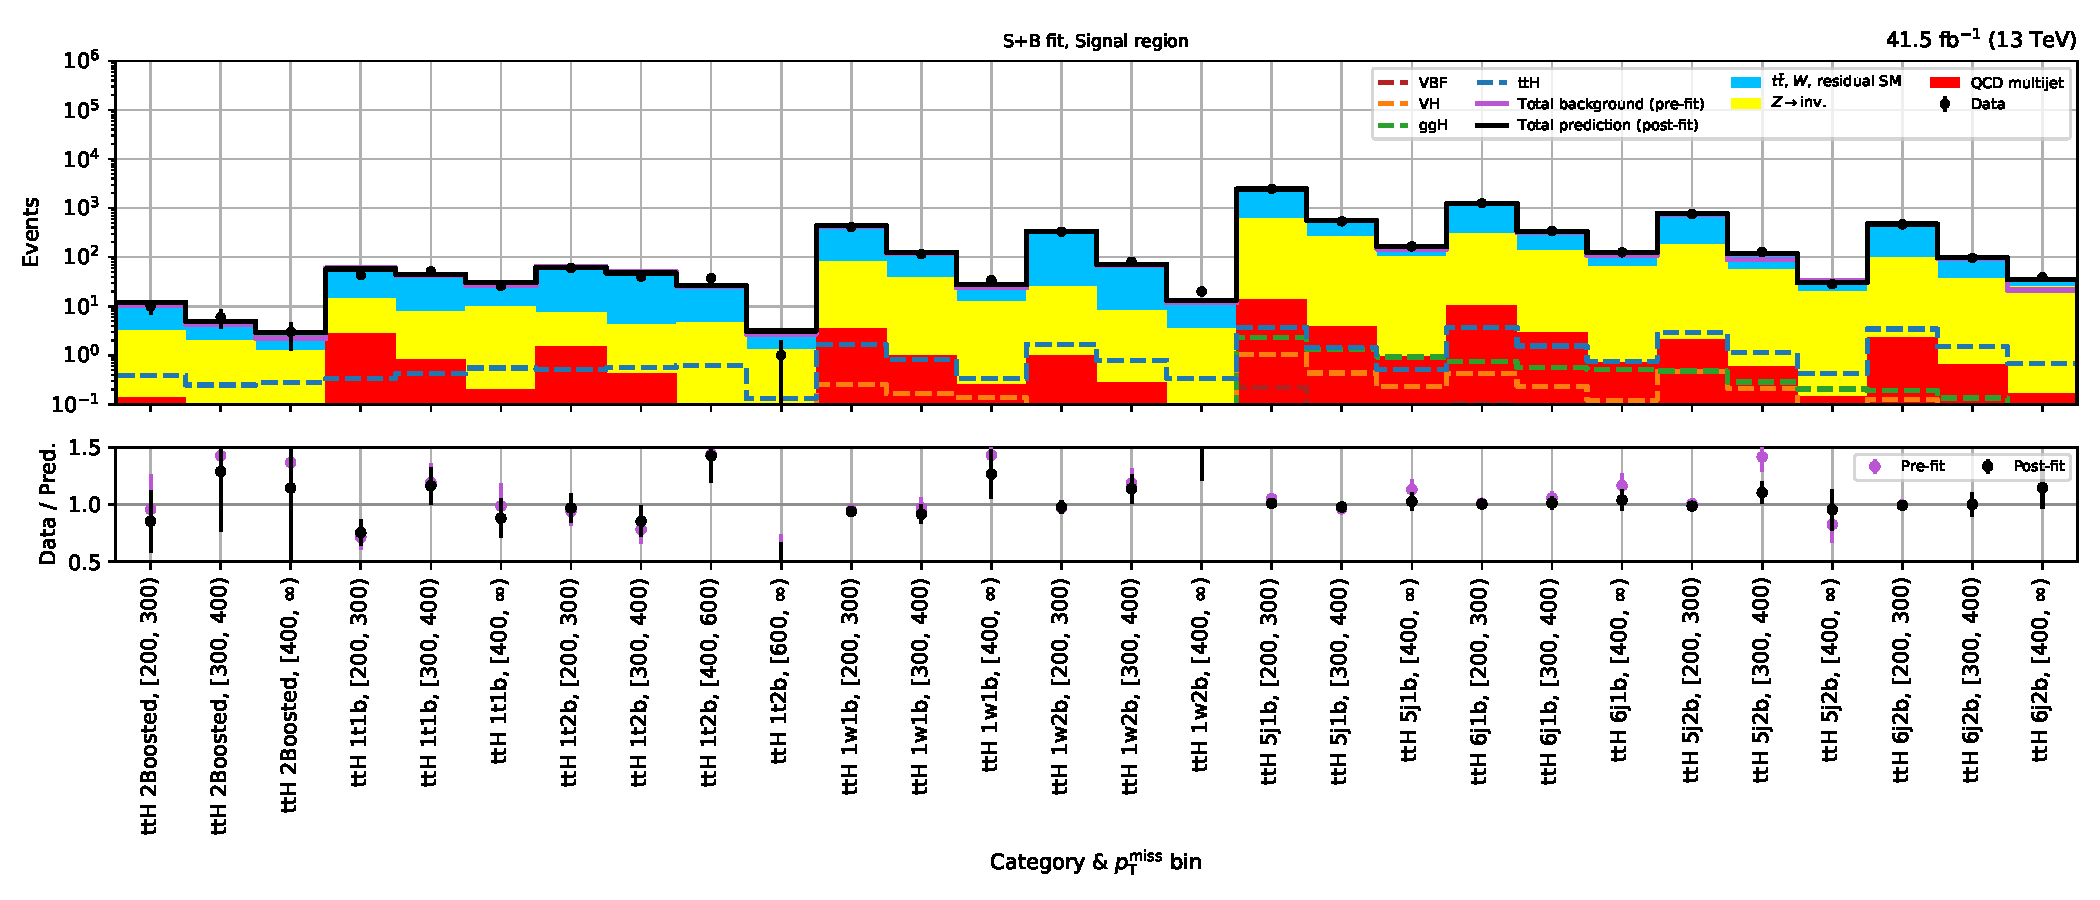
\includegraphics[width=\textwidth]{figures/mountain_ranges/2017/ttH/SR_tree_fit_s-abs_values_ttH_cats.pdf}
        \caption{\ttH --- 2017}
    \end{subfigure}

    \begin{subfigure}[b]{0.9\textwidth}
        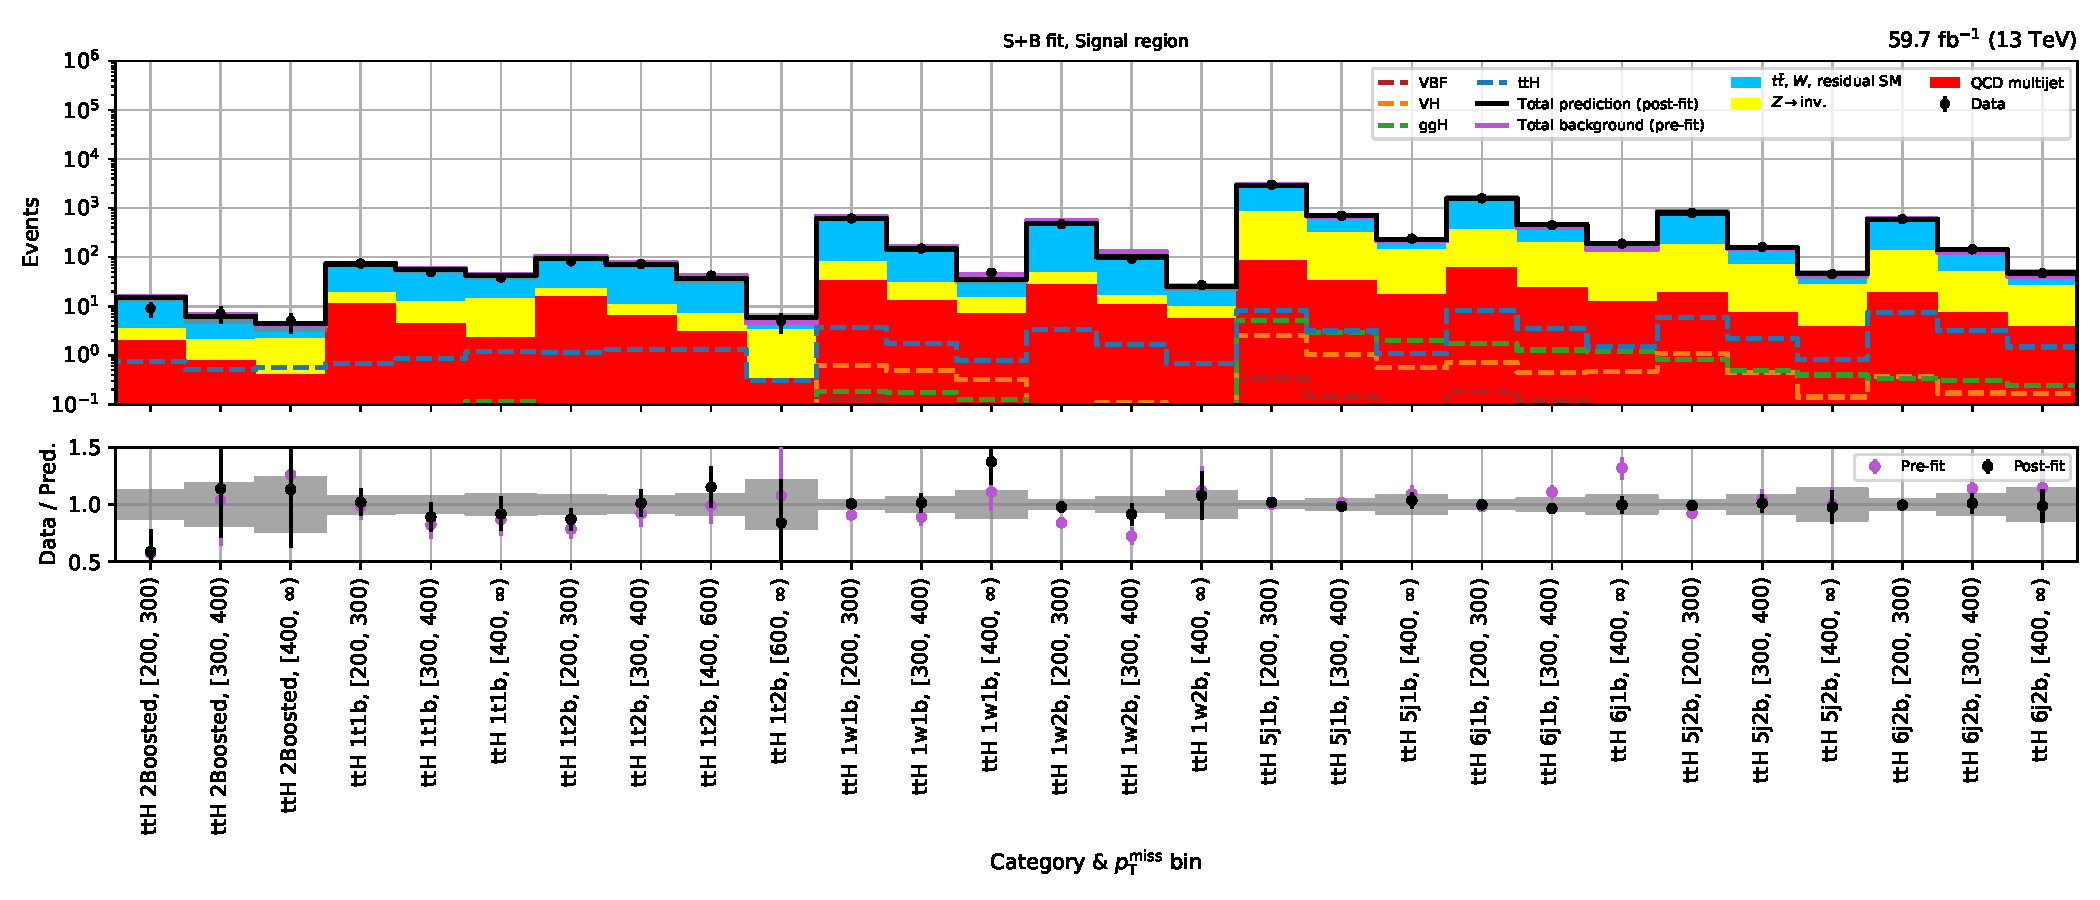
\includegraphics[width=\textwidth]{figures/mountain_ranges/2018/ttH/SR_tree_fit_s-abs_values_ttH_cats.pdf}
        \caption{\ttH --- 2018}
    \end{subfigure}
    \caption[Pre-fit and post-fit yields in the signal region for every \ttH category and \ptmiss bin in each year of Run-2]{Pre-fit and post-fit yields in the signal region for every \ttH category and \ptmiss bin in each year of Run-2. ``Pre-fit'' refers to outcome of the control region-only prediction.}
    \label{fig:htoinv_mountain_range_ttH_SR_Postfit}
\end{figure}

It is evident from the distributions that the fit succeeds in most cases to match the signal and background to the data within uncertainties. Relatively few bins contain a post-fit data/prediction ratio largely different from unity. Sizeable deviations are seen only in the \ttH boosted categories which are statistically limited. In 2016, a general over-prediction of background is seen, corrected for the most part by the fit. The pre-fit ratio is overall better in 2016 than in the other years; the effect of pre-firing was less severe than in 2017. Both of the later years suffered from additional problems such as noise in the \acrshort{ecal} end caps in 2017---affecting \ttH more given its high jet multiplicity---and the HEM Issue in 2018 that largely affects \glspl{jet}, and therefore \ptvecmiss. Techniques were employed to mitigate the problems, but residual mis-modelling may still be present.

\acrshort{qcd} multijet is a somewhat large background in several of the categories despite the \mindphi, \omegaTilde, and \gls{bjet}/boosted object requirements. Even though they are designed to reject a significant fraction of the multijet background, the high cross section of the process leads to a noticeable contribution. \acrshort{qcd} comprises roughly 2--3\,\% of the total background in the resolved categories. However, at low \ptmiss in the boosted categories, its contribution is as high as approximately 10\,\%.

These post-fit distributions translate directly into the upper limit on \BRHinvFull. Fig.~\ref{fig:htoinv_limit_ttH} showcases the limit and profile likelihood scan for the \ttH channel in each data taking year individually and the combination over the full Run-2 dataset. Limits broken down by category in each year are presented in Fig.~\ref{fig:htoinv_limit_ttH_per_year}.

\begin{figure}[htbp]
    \centering
    \begin{subfigure}[t]{0.49\textwidth}    % top align since axis labels are larger for likelihood
        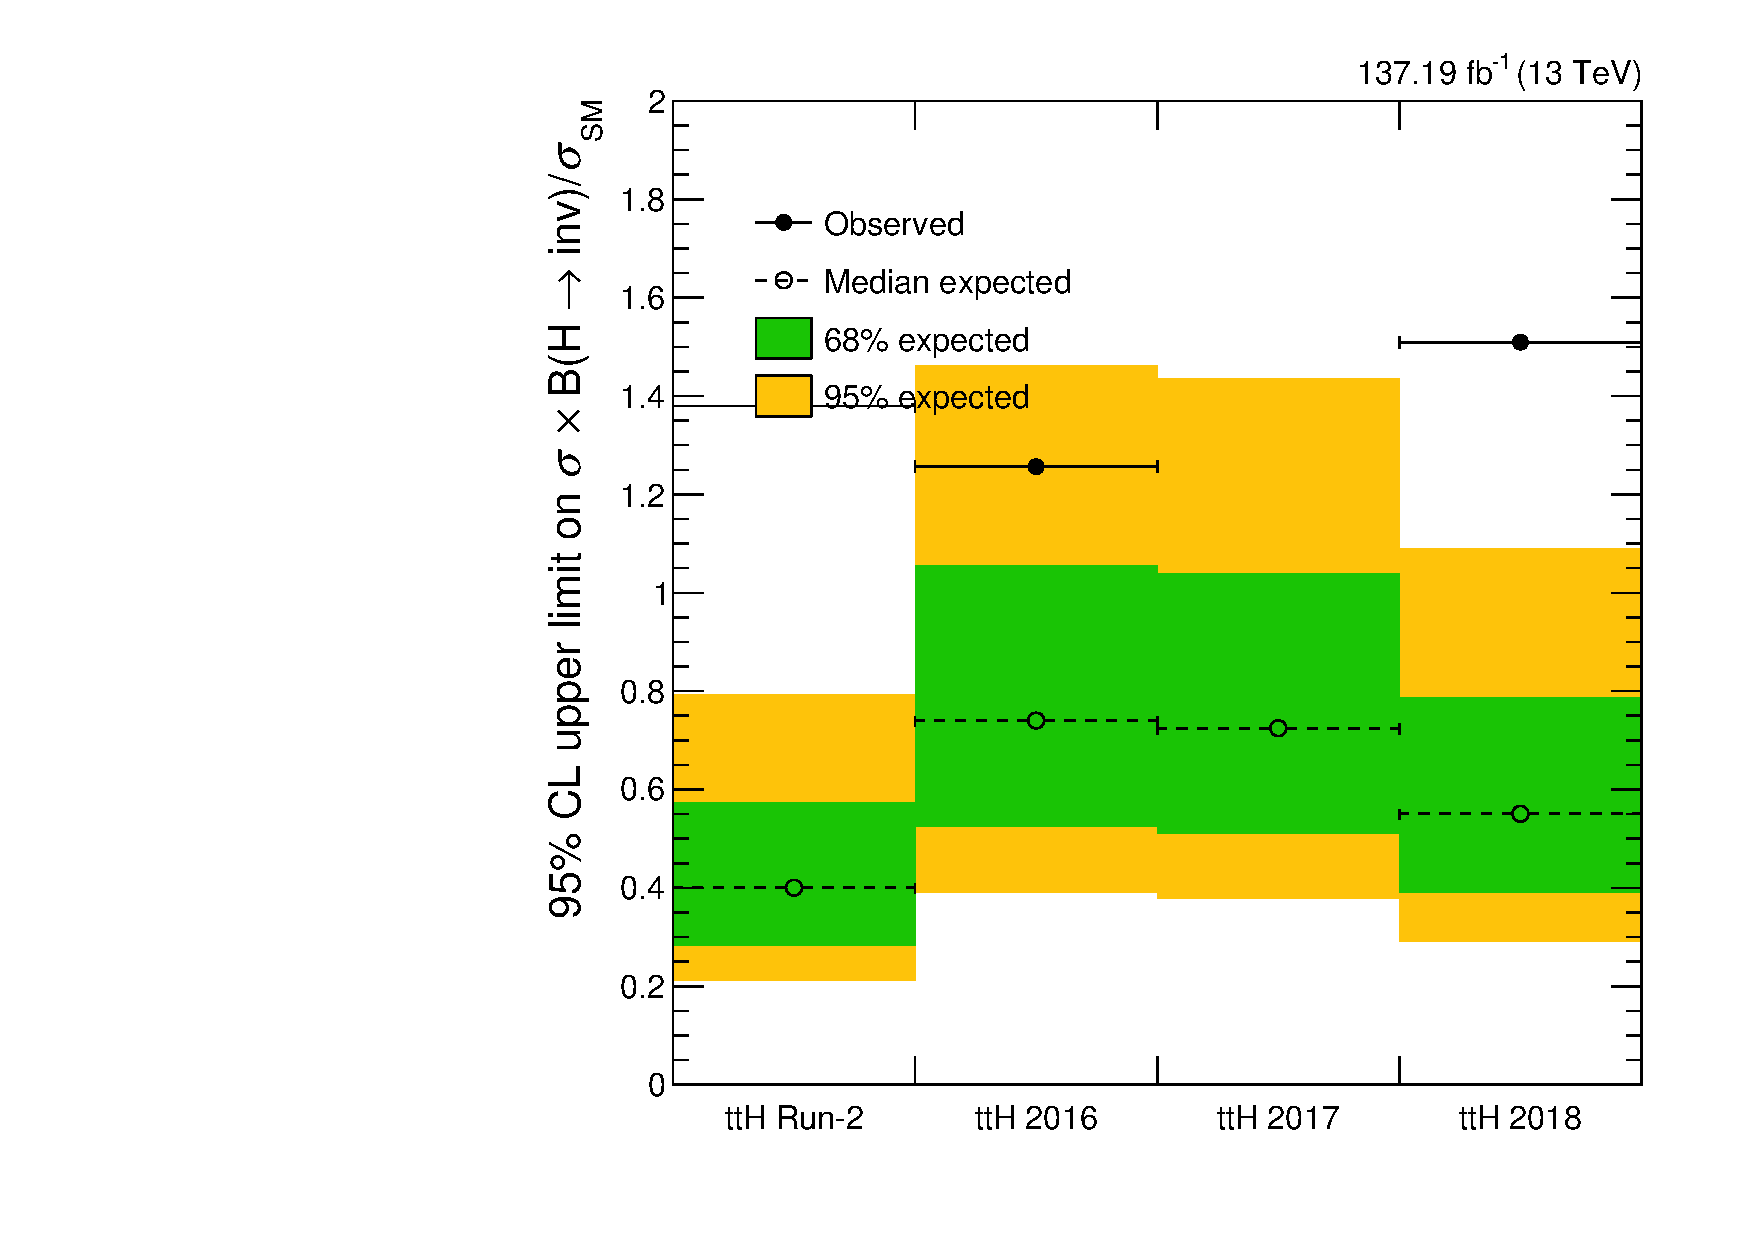
\includegraphics[width=\textwidth]{figures/limits/ttH/limit_Run2_ttH.pdf}
        \caption{Limit --- \ttH}
    \end{subfigure}
    \hfill
    \begin{subfigure}[t]{0.49\textwidth}
        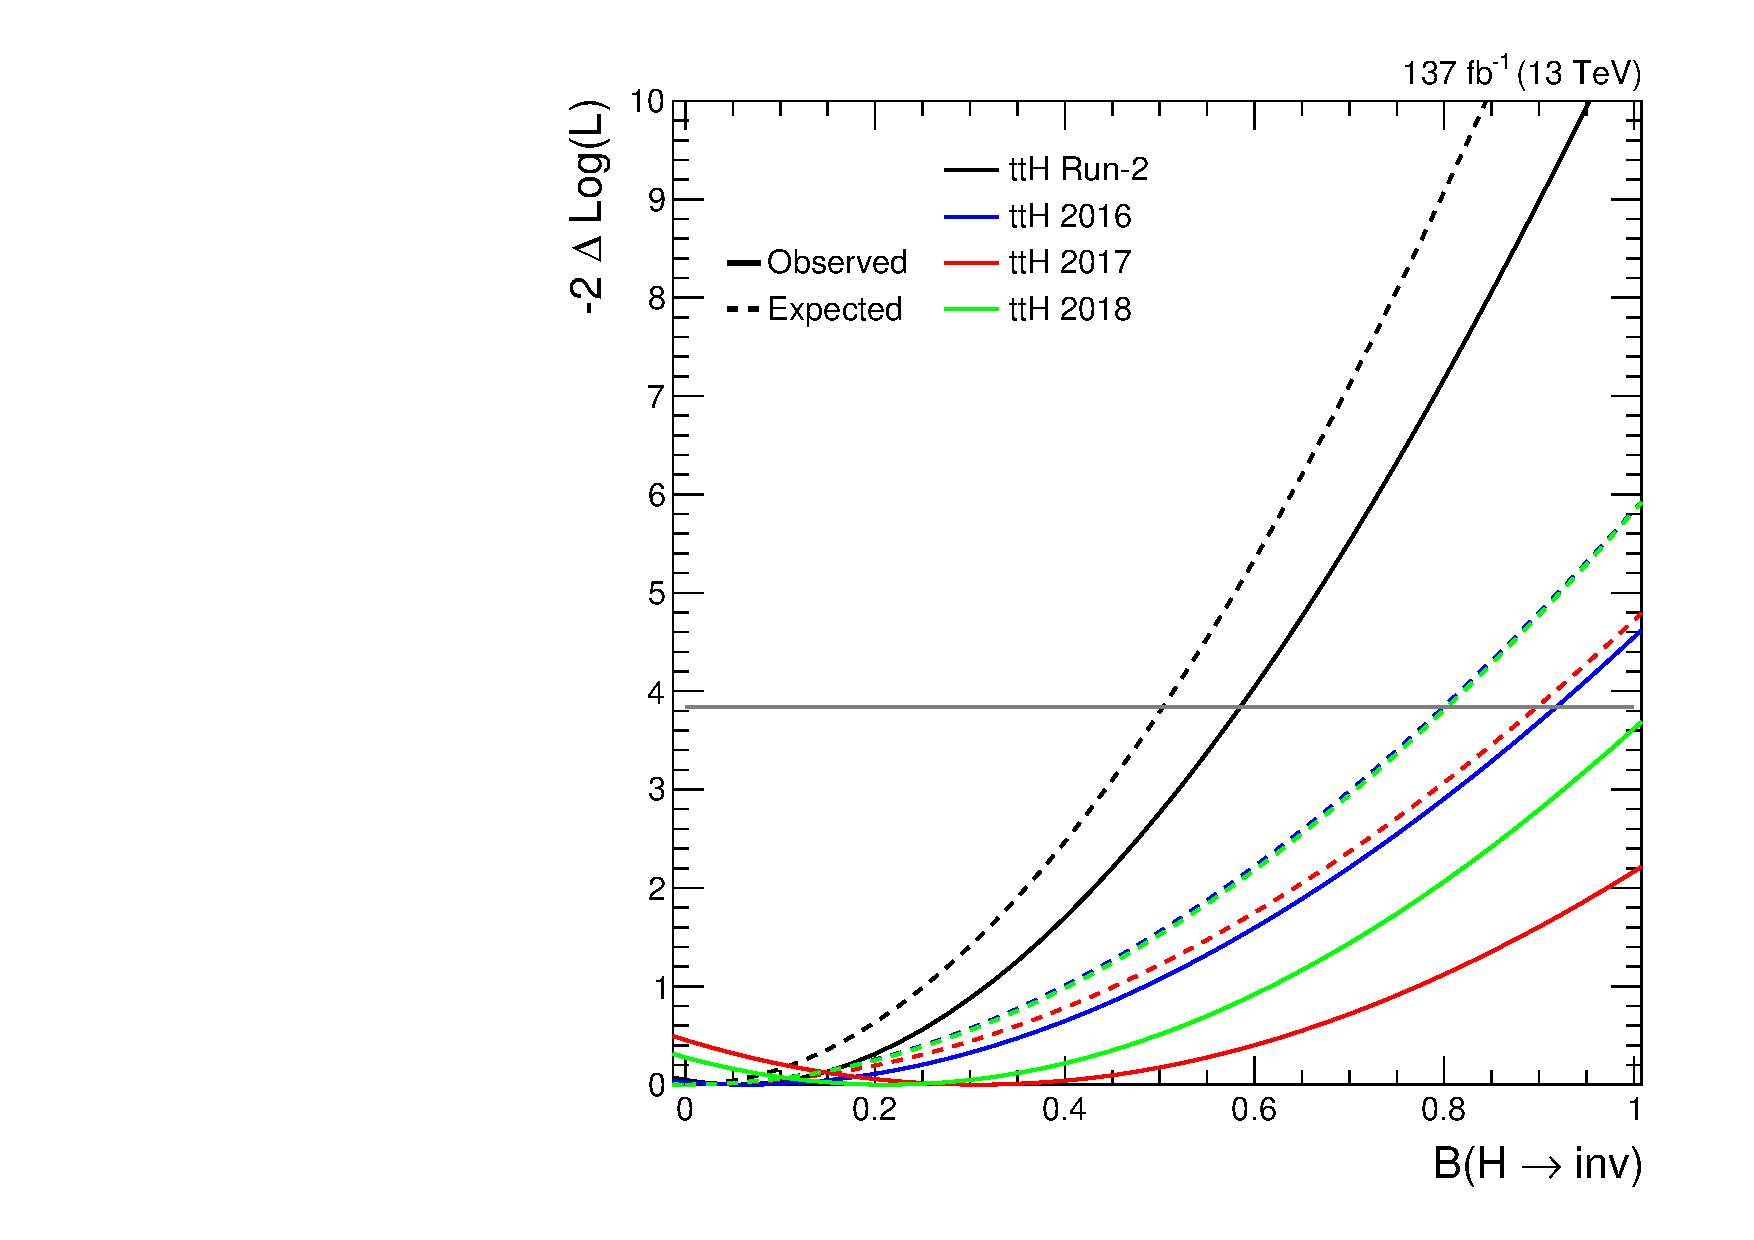
\includegraphics[width=\textwidth]{figures/likelihood_scan/profile_likelihood_scan_Run2_ttH.pdf}
        \caption{Profile likelihood --- \ttH}
    \end{subfigure}
    \caption[Observed and expected 95\,\% CL upper limit on the Higgs boson to invisible state branching fraction $\BRof{\higgstoinv}$ (left) and the corresponding profile likelihood scan (right) in the \ttH channel]{Observed and expected 95\,\% CL upper limit on the Higgs boson to invisible state branching fraction $\BRof{\higgstoinv}$ (left) and the corresponding profile likelihood scan (right) in the \ttH channel. The result from each data taking period is presented along with their combination.}
    \label{fig:htoinv_limit_ttH}
\end{figure}

The sensitivity landscape is mostly consistent between years, more so for 2017 and 2018 given the similarities in simulation and detector configuration. All of the observations are within the $\text{2}\sigma$ boundaries of the expected limit, with many within $\text{1}\sigma$, demonstrating a consistent picture between the \acrshort{sm} expectation and data. The combined Run-2 limit of 50\,\% expected and 56\,\% observed is more sensitive than the analogous combination from \acrshort{atlas} with 94\,\% observed and 64\,\% expected~\cite{ATLAS:2020kdi}.\footnote{All comparisons are evaluated at the 95\,\% confidence level, unless stated otherwise.} Within \acrshort{cms}, comparisons may only be drawn with the preliminary result from the 2016 dataset~\cite{CMS-PAS-HIG-18-008}; a result of 85\,\% was observed and 73\,\% expected in the 0-lepton channel. From this thesis, a similar sensitivity is achieved with 88\,\% observed and 80\,\% expected. The greater sensitivity in the preliminary result could be explained by a number of reasons. Additional systematic uncertainties were included in this analysis such as the \acrshort{qcd} scale for top quark processes, \acrlong{jer}, and those associated with the \acrshort{nlo} corrections to $\PVec \plusjets$ backgrounds.

By category, those targeting the boosted topologies are the most sensitive to the invisible decays of the Higgs boson (see Fig.~\ref{fig:htoinv_limit_likelihood_boosted_resolved_cats_Run2}). Given the purity of these categories, it is understandable why. Despite greater statistical power in the resolved regime, systematic uncertainties would have a larger absolute effect and possibly conceal signal due to their size. These result in generally weaker limits than the boosted categories.

The profile likelihood scans illustrate how the likelihood function for the fit over a set of categories evolves with the upper limit on branching ratio. The horizontal line $-\text{2}\Delta \ln(\likelihood) = \text{3.84}$ represents the 95\,\% confidence level. It can therefore be seen that the intersection of a dashed curve with the line is equal to the median expected limit, and the intersection of a solid curve with it equals the measured observed limit. Indicative of the stability and health of the fit, the likelihood scans in Fig.~\ref{fig:htoinv_limit_ttH} are satisfactory with minima near $\BR = \text{0}$, rising smoothly either side of it.


%=========================================================


\subsection{Results from the \texorpdfstring{\VH}{VH} channel}
\label{subsec:htoinv_results_VH}

Distributions of the prediction from the signal plus background fit to data, for 2016, 2017, and 2018, are displayed in Fig.~\ref{fig:htoinv_mountain_range_VH_SR_Postfit}. The \acrshort{sm} prediction from the \gls{CR}-only fit (with event yields in Sec.~\ref{subsec:yield_tables_SR_CR_only_fit}) is overlaid for comparison. Corresponding figures of the \glspl{CR} resulting from the \gls{CR}-only fit are given in Sec.~\ref{sec:pre_post_fit_plots_VH_CRs}.

\begin{figure}[htbp]
    \centering
    \begin{subfigure}[b]{0.9\textwidth}
        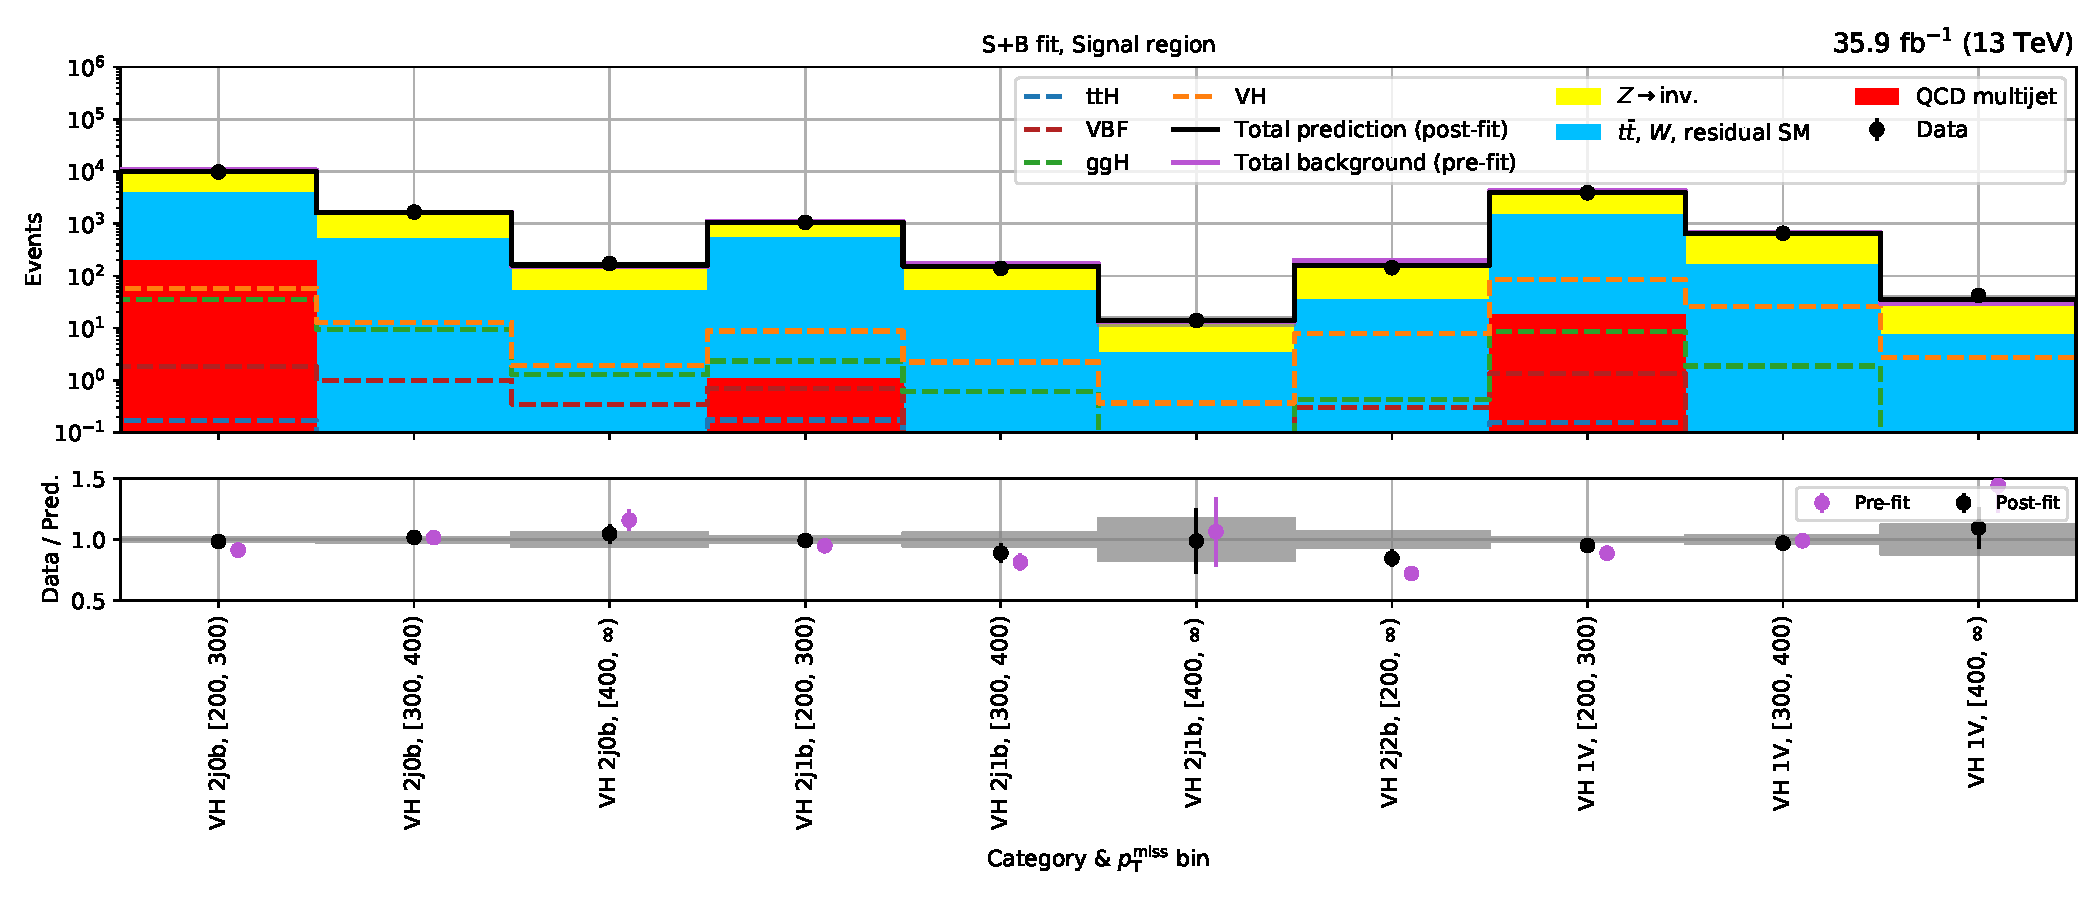
\includegraphics[width=\textwidth]{figures/mountain_ranges/2016/VH/SR_tree_fit_s-abs_values_VH_cats.pdf}
        \caption{\VH --- 2016}
    \end{subfigure}

    \begin{subfigure}[b]{0.9\textwidth}
        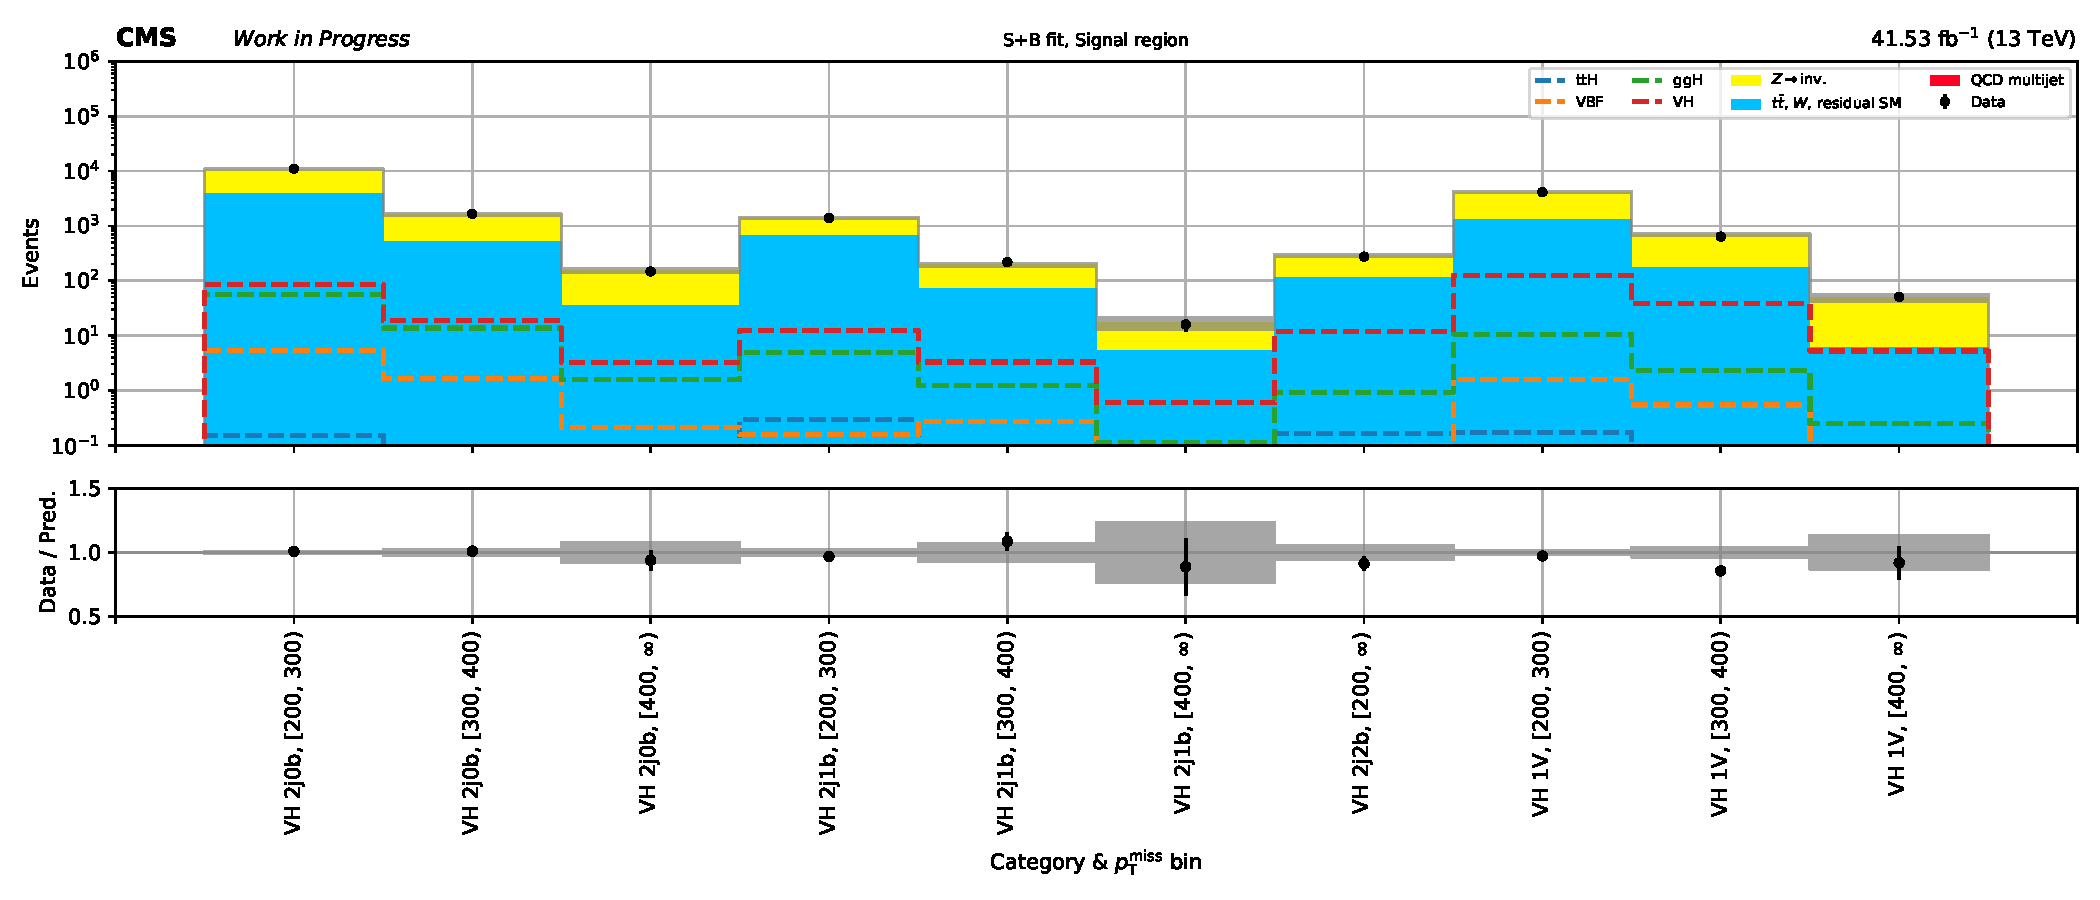
\includegraphics[width=\textwidth]{figures/mountain_ranges/2017/VH/SR_tree_fit_s-abs_values_VH_cats.pdf}
        \caption{\VH --- 2017}
    \end{subfigure}

    \begin{subfigure}[b]{0.9\textwidth}
        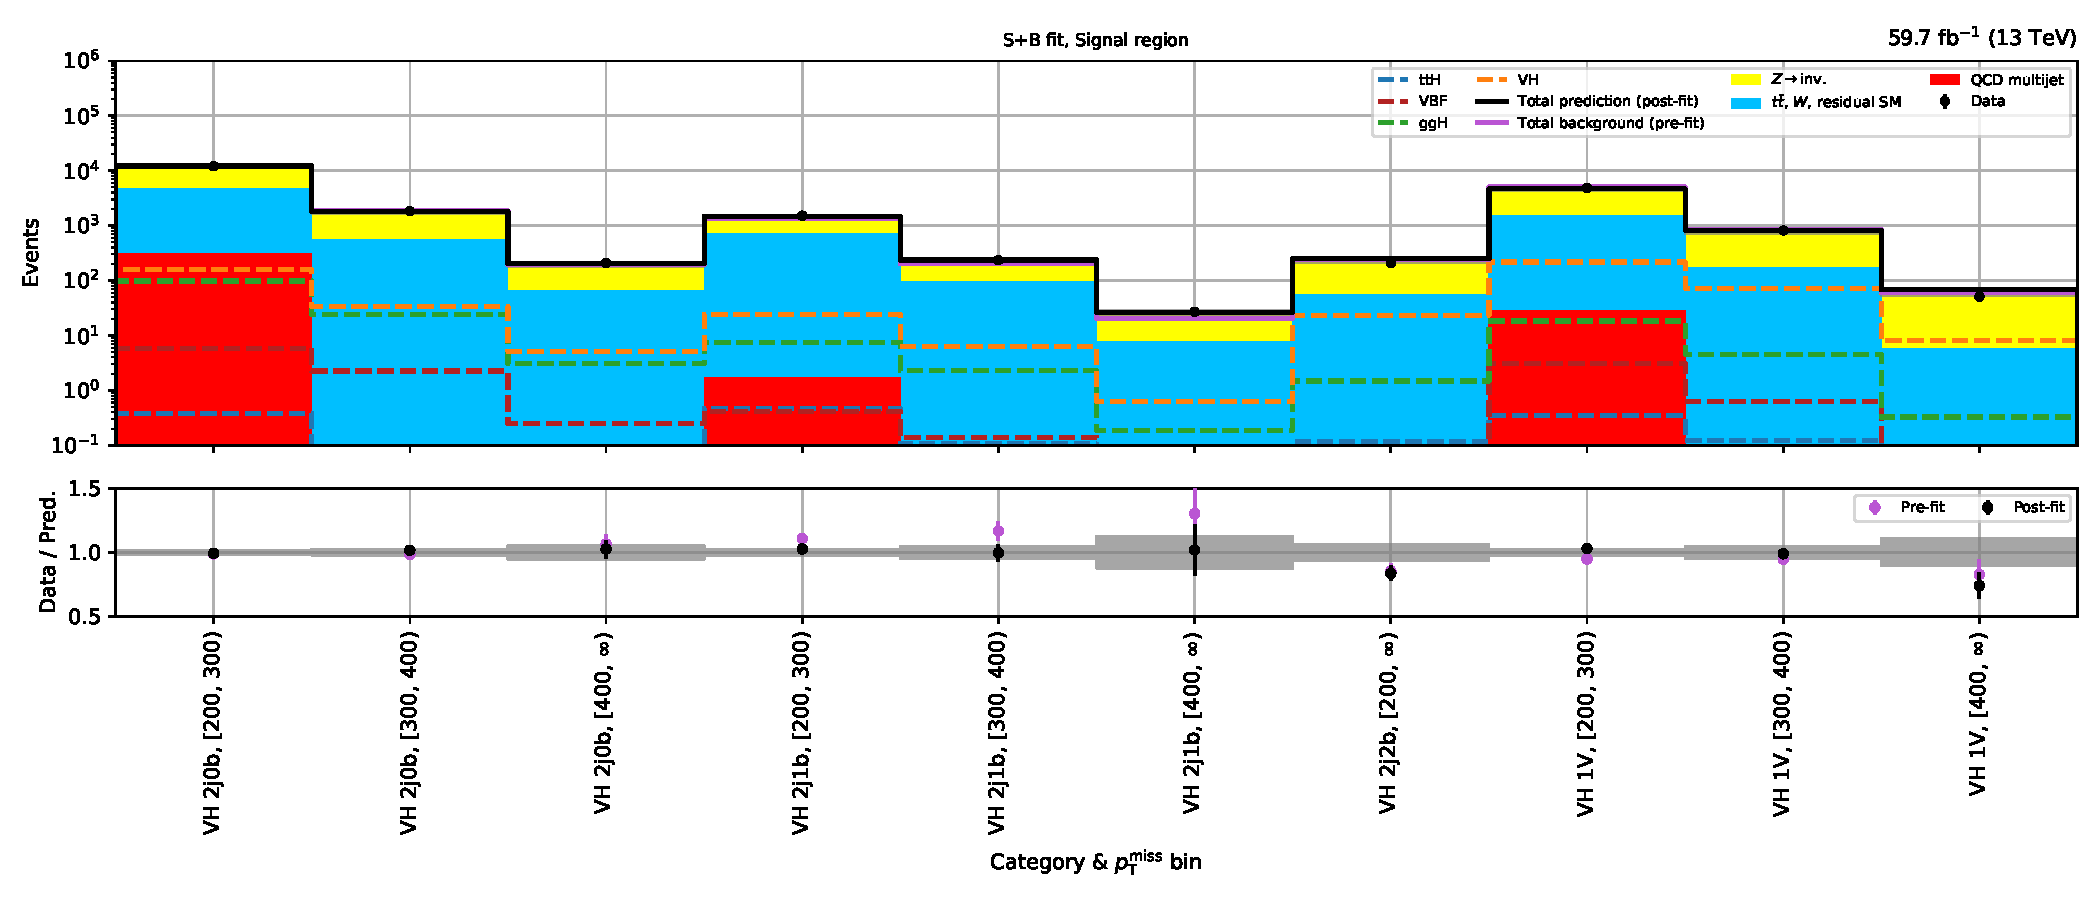
\includegraphics[width=\textwidth]{figures/mountain_ranges/2018/VH/SR_tree_fit_s-abs_values_VH_cats.pdf}
        \caption{\VH --- 2018}
    \end{subfigure}
    \caption[Pre-fit and post-fit yields in the signal region for every \VH category and \ptmiss bin in each year of Run-2]{Pre-fit and post-fit yields in the signal region for every \VH category and \ptmiss bin in each year of Run-2. ``Pre-fit'' refers to outcome of the control region-only prediction.}
    \label{fig:htoinv_mountain_range_VH_SR_Postfit}
\end{figure}

The \VH topology is dominated by the irreducible \ztonunupjets background, followed by lost lepton, and finally a small amount of \acrshort{qcd} multijet. Especially with the \gls{bjet}/boosted object requirements and dijet signature coupled to a small mass window around the electroweak bosons, it is a percent-level background in the bins where it appears. The post-fit prediction agrees with the data well in most cases, demonstrating an adequate description and leaving little room for signal to be inflated. An exception is the 1V category in 2018 whose observation is much larger than in the preceding years. The observed limits for 2j0b and 2j1b also fall close to, if not slightly outside, the $\text{2}\sigma$ bound of the expected limit in 2017 and 2018.

Fig.~\ref{fig:htoinv_limit_VH} showcases the expected and observed limits for the \VH channel in each year and for the Run-2 combination. Limits for the individual categories can be found in Fig.~\ref{fig:htoinv_limit_VH_per_year}.

\begin{figure}[htbp]
    \centering
    \begin{subfigure}[t]{0.49\textwidth}
        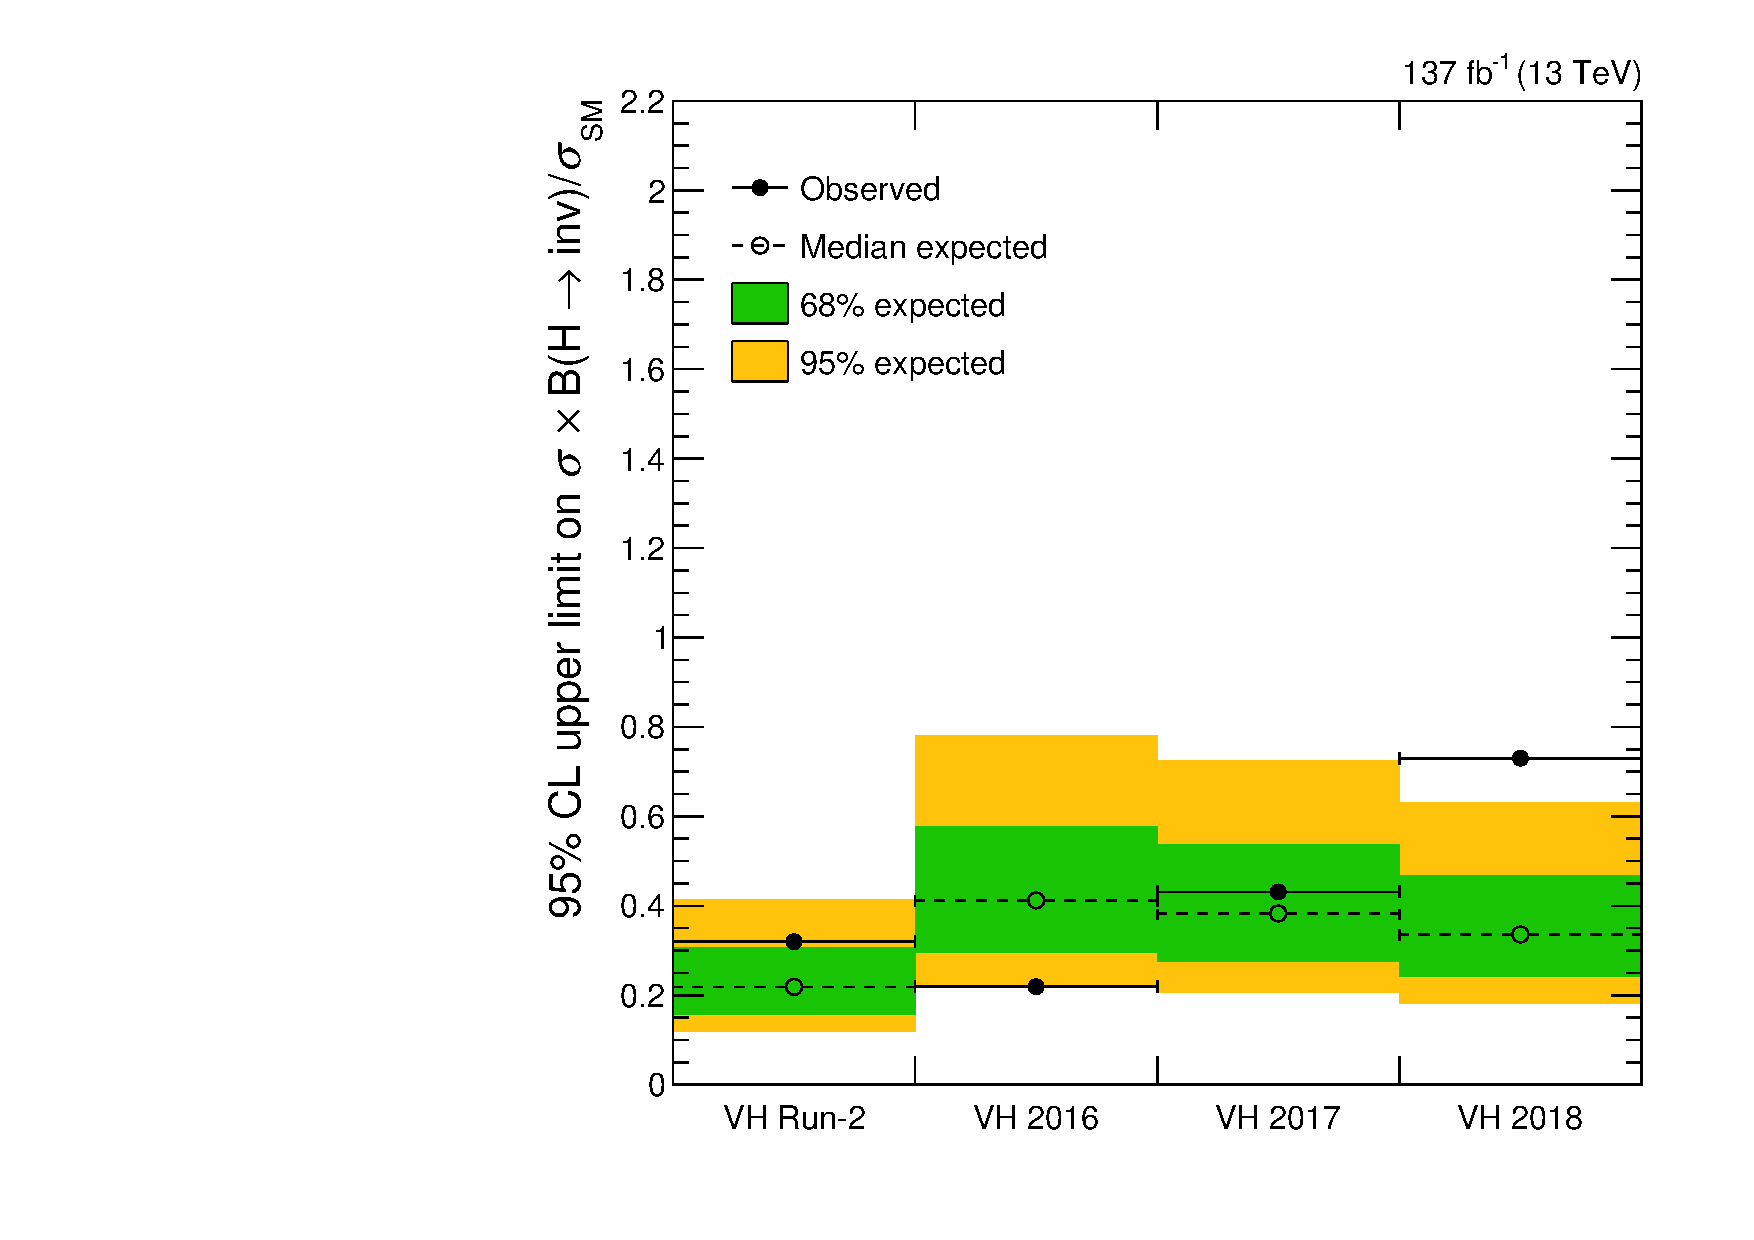
\includegraphics[width=\textwidth]{figures/limits/VH/limit_Run2_VH.pdf}
        \caption{Limit --- \VH}
    \end{subfigure}
    \hfill
    \begin{subfigure}[t]{0.49\textwidth}
        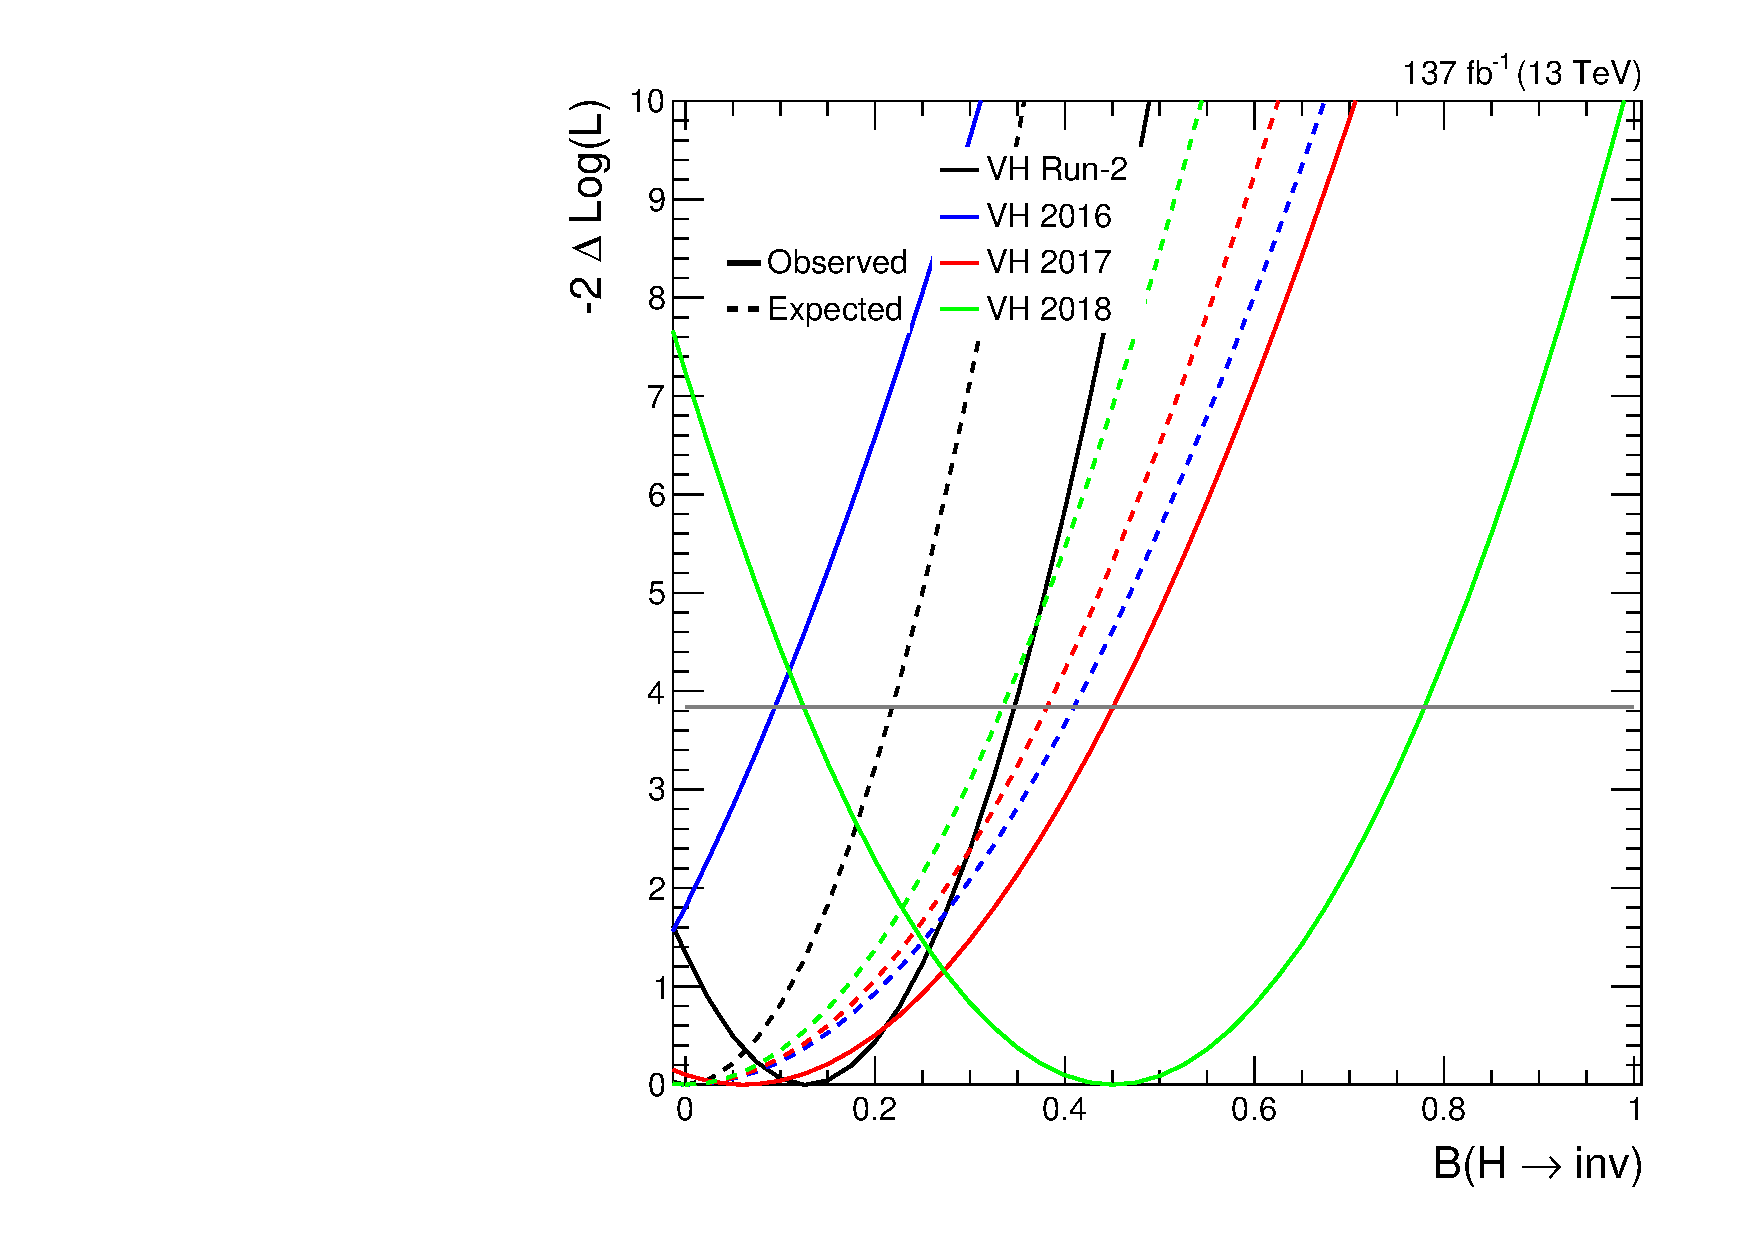
\includegraphics[width=\textwidth]{figures/likelihood_scan/profile_likelihood_scan_Run2_VH.pdf}
        \caption{Profile likelihood --- \VH}
    \end{subfigure}
    \caption[Observed and expected 95\,\% CL upper limit on the Higgs boson to invisible state branching fraction $\BRof{\higgstoinv}$ (left) and the corresponding profile likelihood scan (right) in the \VH channel]{Observed and expected 95\,\% CL upper limit on the Higgs boson to invisible state branching fraction $\BRof{\higgstoinv}$ (left) and the corresponding profile likelihood scan (right) in the \VH channel. The result from each data taking period is presented along with their combination.}
    \label{fig:htoinv_limit_VH}
\end{figure}

The obtained limits demonstrate that the sensitivity of the \VH topology to \higgstoinv is second only to \acrshort{vbf}. Fig.~\ref{fig:htoinv_limit_VH_per_year} makes apparent that the sensitivity of \VH within a given year, and overall, is driven by the 1V category. It is closely followed by 2j0b (rich in $\HepProcess{\PVec \to \Pquark\APquark}$) and 2j2b (targeting $\HepProcess{\PZ \to \Pqb\Paqb}$). 2j1b lags behind as it relies on a \gls{bjet} either being falsely tagged by the \deepcsv algorithm or missed by it. Fluctuations between years average to yield a full Run-2 observed limit of 32\,\% and expected of 22\,\%---a very competitive result in the invisible Higgs landscape for a single production mode. Contributions to the overall limit from the boosted (1V) and resolved categories can be seen in Fig.~\ref{fig:htoinv_limit_likelihood_boosted_resolved_cats_Run2}. While 1V contributes most to the expected limit, the resolved categories collectively drive the observed limit.

For comparisons to public results, there are no full Run-2 hadronic $\VH(\higgstoinv)$ searches or interpretations. Results from both \acrshort{atlas} and \acrshort{cms} are, however, available using 2016 data. The latter is a mono-\PVec search comparable to the 1V category from this thesis. The \acrshort{atlas} \VH result found an observed limit of 83\,\% and expected of 58\,\%~\cite{Aaboud:2018xdl}, while from \acrshort{cms} they were 50\,\% and 48\,\%, respectively~\cite{Sirunyan:2017jix}. From this thesis, an observed limit of 67\,\% and expected of 55\,\% is obtained for the 1V category (see Fig.~\ref{fig:htoinv_limit_VH_2016}). Sensitivity is better than that of \acrshort{atlas} but worse than the \acrshort{cms} result with solely the 2016 dataset. Differences in signal modelling are likely a factor. Older simulated signal has been found to use fixed factorisation scales at the \PW or \PH mass as opposed to the running scales in newer samples such as those used in this thesis; consequently, a harder Higgs boson \pt (i.e., \ptmiss) spectrum is exhibited in the older samples. Dissimilarities such as these make direct comparisons to previous results more difficult.

% Info about signal scale from 2016: https://indico.cern.ch/event/978146/contributions/4120060/attachments/2149295/3623502/2020-11-20_monov_update%2B.pdf

The limits per year in Fig.~\ref{fig:htoinv_limit_VH} are inconsistent to some degree, with an observation slightly below the $\text{2}\sigma$ boundary of the expected limit in 2016, correspondence in 2017, and an excess in 2018. In 2018, the observed limit is noticeably worse than in the preceding two. Inference from Figs.~\ref{fig:htoinv_mountain_range_VH_2018_single_lep_CRs} and \ref{fig:htoinv_mountain_range_VH_2018_dilep_photon_CRs} suggests it is due the over-prediction of simulation in all of the leptonic \glspl{CR} of the 1V category, consequently scaling down the background in the signal region. As to the root cause of the discrepancy, it may be residual effects of the HEM Issue, or a difference in performance of the \deepakeight algorithm between data and \acrshort{mc} not fully captured by the scale factors. The 2j0b observation is also just outside the $\text{2}\sigma$ interval, further affecting the fit to the whole channel. Reassuringly, the expected limits per year are stable and as assumed (sensitivity improving each year, following the trend in integrated luminosity). No issues are found with the likelihood scans, either.


%=========================================================


\subsection{Combined results}
\label{subsec:htoinv_combined_results}

The combined upper limit on $\BRHinvFull$ from combining the \ttH and \VH channels for the full Run-2 dataset is illustrated in Fig.~\ref{fig:htoinv_limit_likelihood_Run2_per_cat}. Profile likelihood scans are presented opposite the limits.

\begin{figure}[htbp]
    \centering
    \begin{subfigure}[t]{0.49\textwidth}
        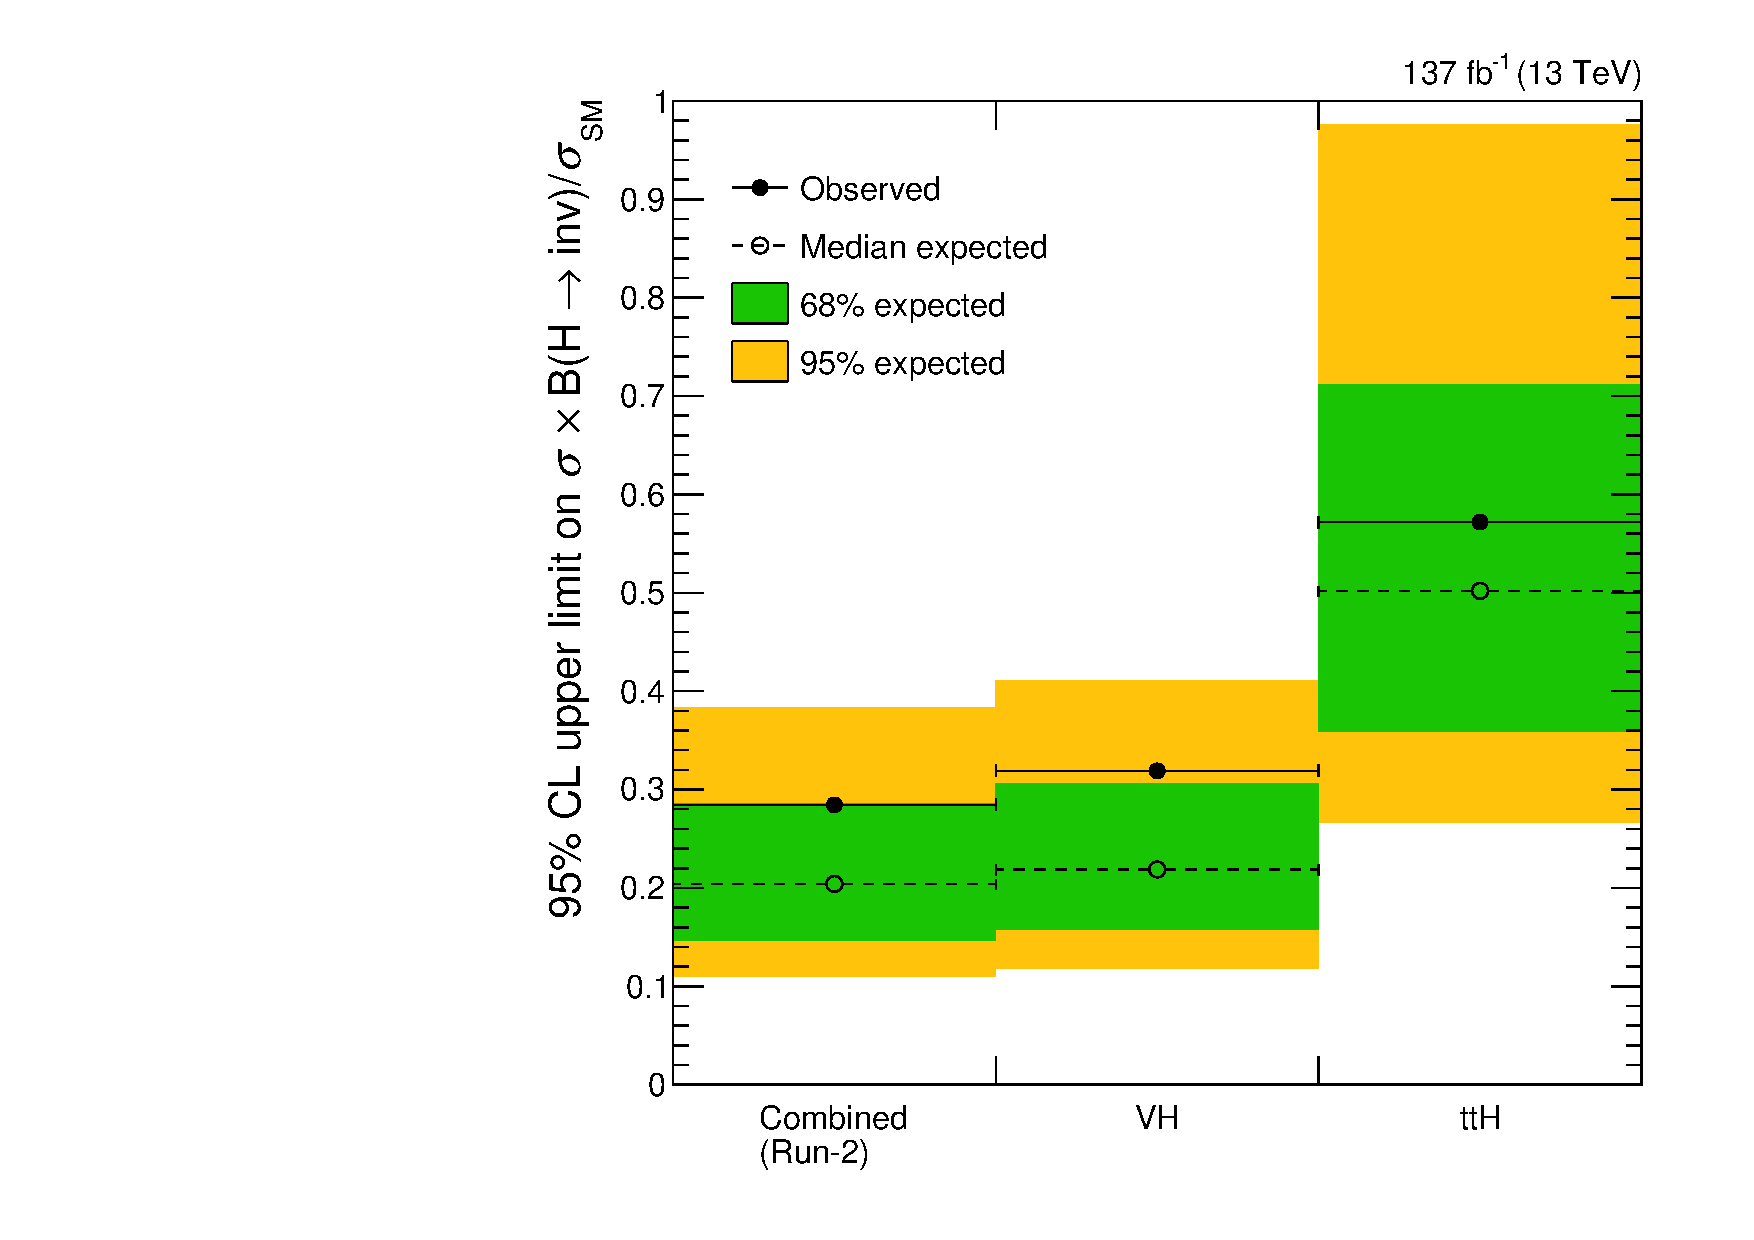
\includegraphics[width=\textwidth]{figures/limits/full_Run2/limit_Run2_comb_per_cat.pdf}
        \caption{Limit --- Run-2}
    \end{subfigure}
    \hfill
    \begin{subfigure}[t]{0.49\textwidth}
        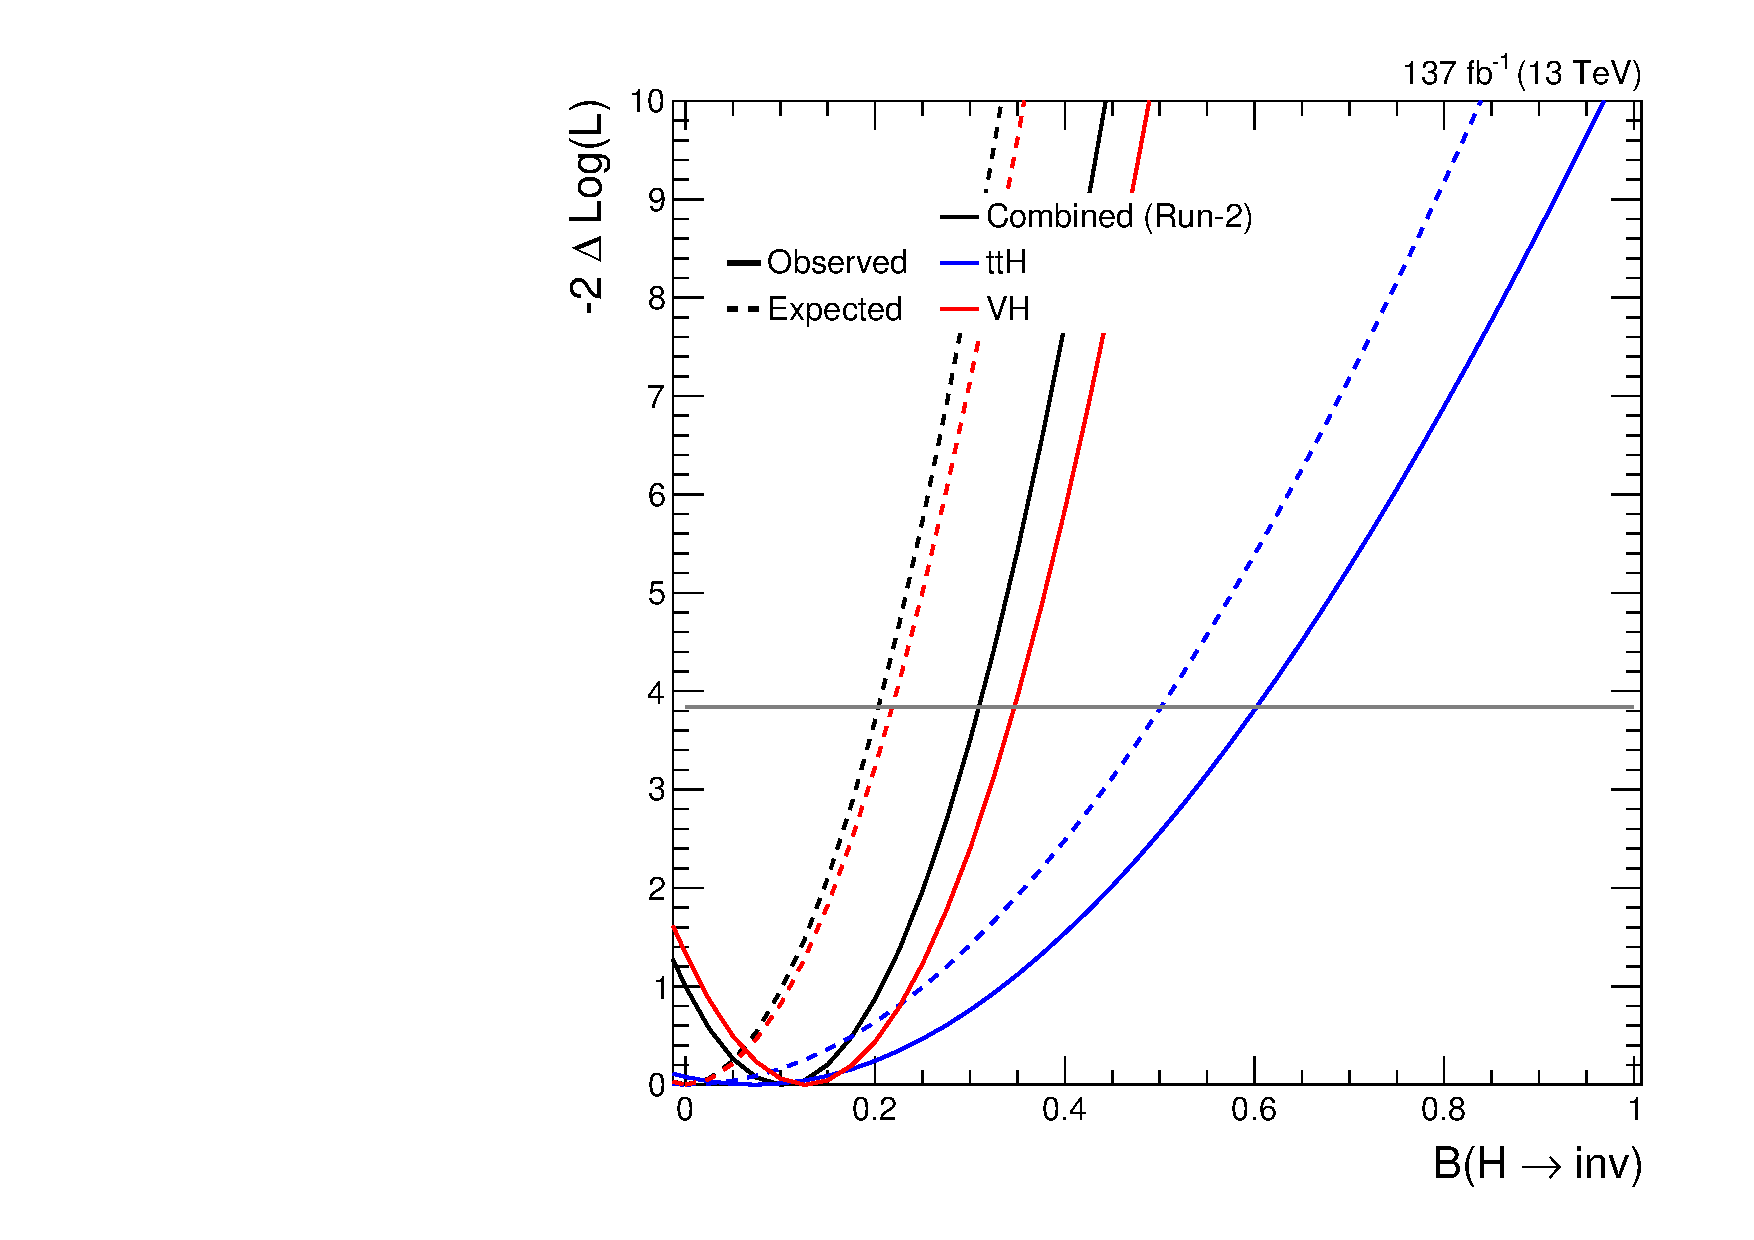
\includegraphics[width=\textwidth]{figures/likelihood_scan/profile_likelihood_scan_Run2_per_cat.pdf}
        \caption{Profile likelihood --- Run-2}
    \end{subfigure}
    \caption[Observed and expected 95\,\% CL upper limit on the Higgs boson to invisible state branching fraction $\BRof{\higgstoinv}$ and the corresponding profile likelihood scan, for both the individual categories, as well as the combination of them, for the full Run-2 dataset]{Observed and expected 95\,\% CL upper limit on the Higgs boson to invisible state branching fraction $\BRof{\higgstoinv}$ (left) and the corresponding profile likelihood scan (right), for both the individual categories, as well as the combination of them, for the full Run-2 dataset. The \acrlong{sm} Higgs boson with its associated mass and production cross section are assumed.}
    \label{fig:htoinv_limit_likelihood_Run2_per_cat}
\end{figure}

The \VH channel predominantly drives the combined observed and expected sensitivity, with upper limits of 28\,\% and 20\,\%, respectively. Nevertheless, the \ttH category does constrain the combination and reduces the uncertainty bands around the expected limit. Both results are competitive with existing searches, with comparable results with the 2016 dataset to those published by both \acrshort{cms} and \acrshort{atlas}. No full Run-2 combination exists for the \VH channel, so the results in this thesis set the benchmark for future endeavours. The \ttH result with the full Run-2 dataset is stronger than that of \acrshort{atlas}, also setting the standard for later searches to improve upon. Expected limits evolve naturally over the years, consistent with the integrated luminosity. A summary of the observed and median expected limits for both the \ttH and \VH channels, together with their combination, is given in Tab.~\ref{tab:htoinv_limits}.

\begin{table}[htbp]
    \centering
    \begin{tabular}{ccccc}
        \toprule
        Dataset & \ttH & \VH & Combined\\\midrule
        \multirow{2}{*}{2016} & 88\,\% (obs.) & 22\,\% (obs.) & 22\,\% (obs.) \\
        & 80\,\% (exp.) & 41\,\% (exp.) & 36\,\% (exp.) \\
        \midrule
        \multirow{2}{*}{2017} & 115\,\% (obs.) & 43\,\% (obs.) & 42\,\% (obs.) \\
        & 90\,\% (exp.) & 38\,\% (exp.) & 36\,\% (exp.) \\
        \midrule
        \multirow{2}{*}{2018} & 96\,\% (obs.) & 73\,\% (obs.) & 68\,\% (obs.) \\
        & 80\,\% (exp.) & 34\,\% (exp.) & 31\,\% (exp.) \\
        \midrule
        \multirow{2}{*}{Run-2} & 56\,\% (obs.) & 32\,\% (obs.) & \textbf{28\,\% (obs.)} \\
        & 50\,\% (exp.) & 22\,\% (exp.) & \textbf{20\,\% (exp.)} \\
        \bottomrule
    \end{tabular}
    \caption[Observed and median expected upper limits on $\BRof{\higgstoinv}$ at 95\,\% confidence level for each combination of channel and dataset analysed]{Observed and median expected upper limits on $\BRof{\higgstoinv}$ at 95\,\% confidence level for each combination of channel and dataset analysed.}
    \label{tab:htoinv_limits}
\end{table}
